\documentclass{article}

\usepackage{imports}

\title{\bfseries работа на паре \TeX'а}
\author{Михаил Ушаков 7 мат}
\date{\today}

\begin{document}
\maketitle

\begin{itemize}
    \item[] \!\!\!\!\!\!\!\!Картинки
    \item[$\equiv$] Птички
    \item[$\equiv$] Типо квадратики...
\end{itemize}
    
\begin{figure}[ht!]
\begin{multicols}{2}
\hfill
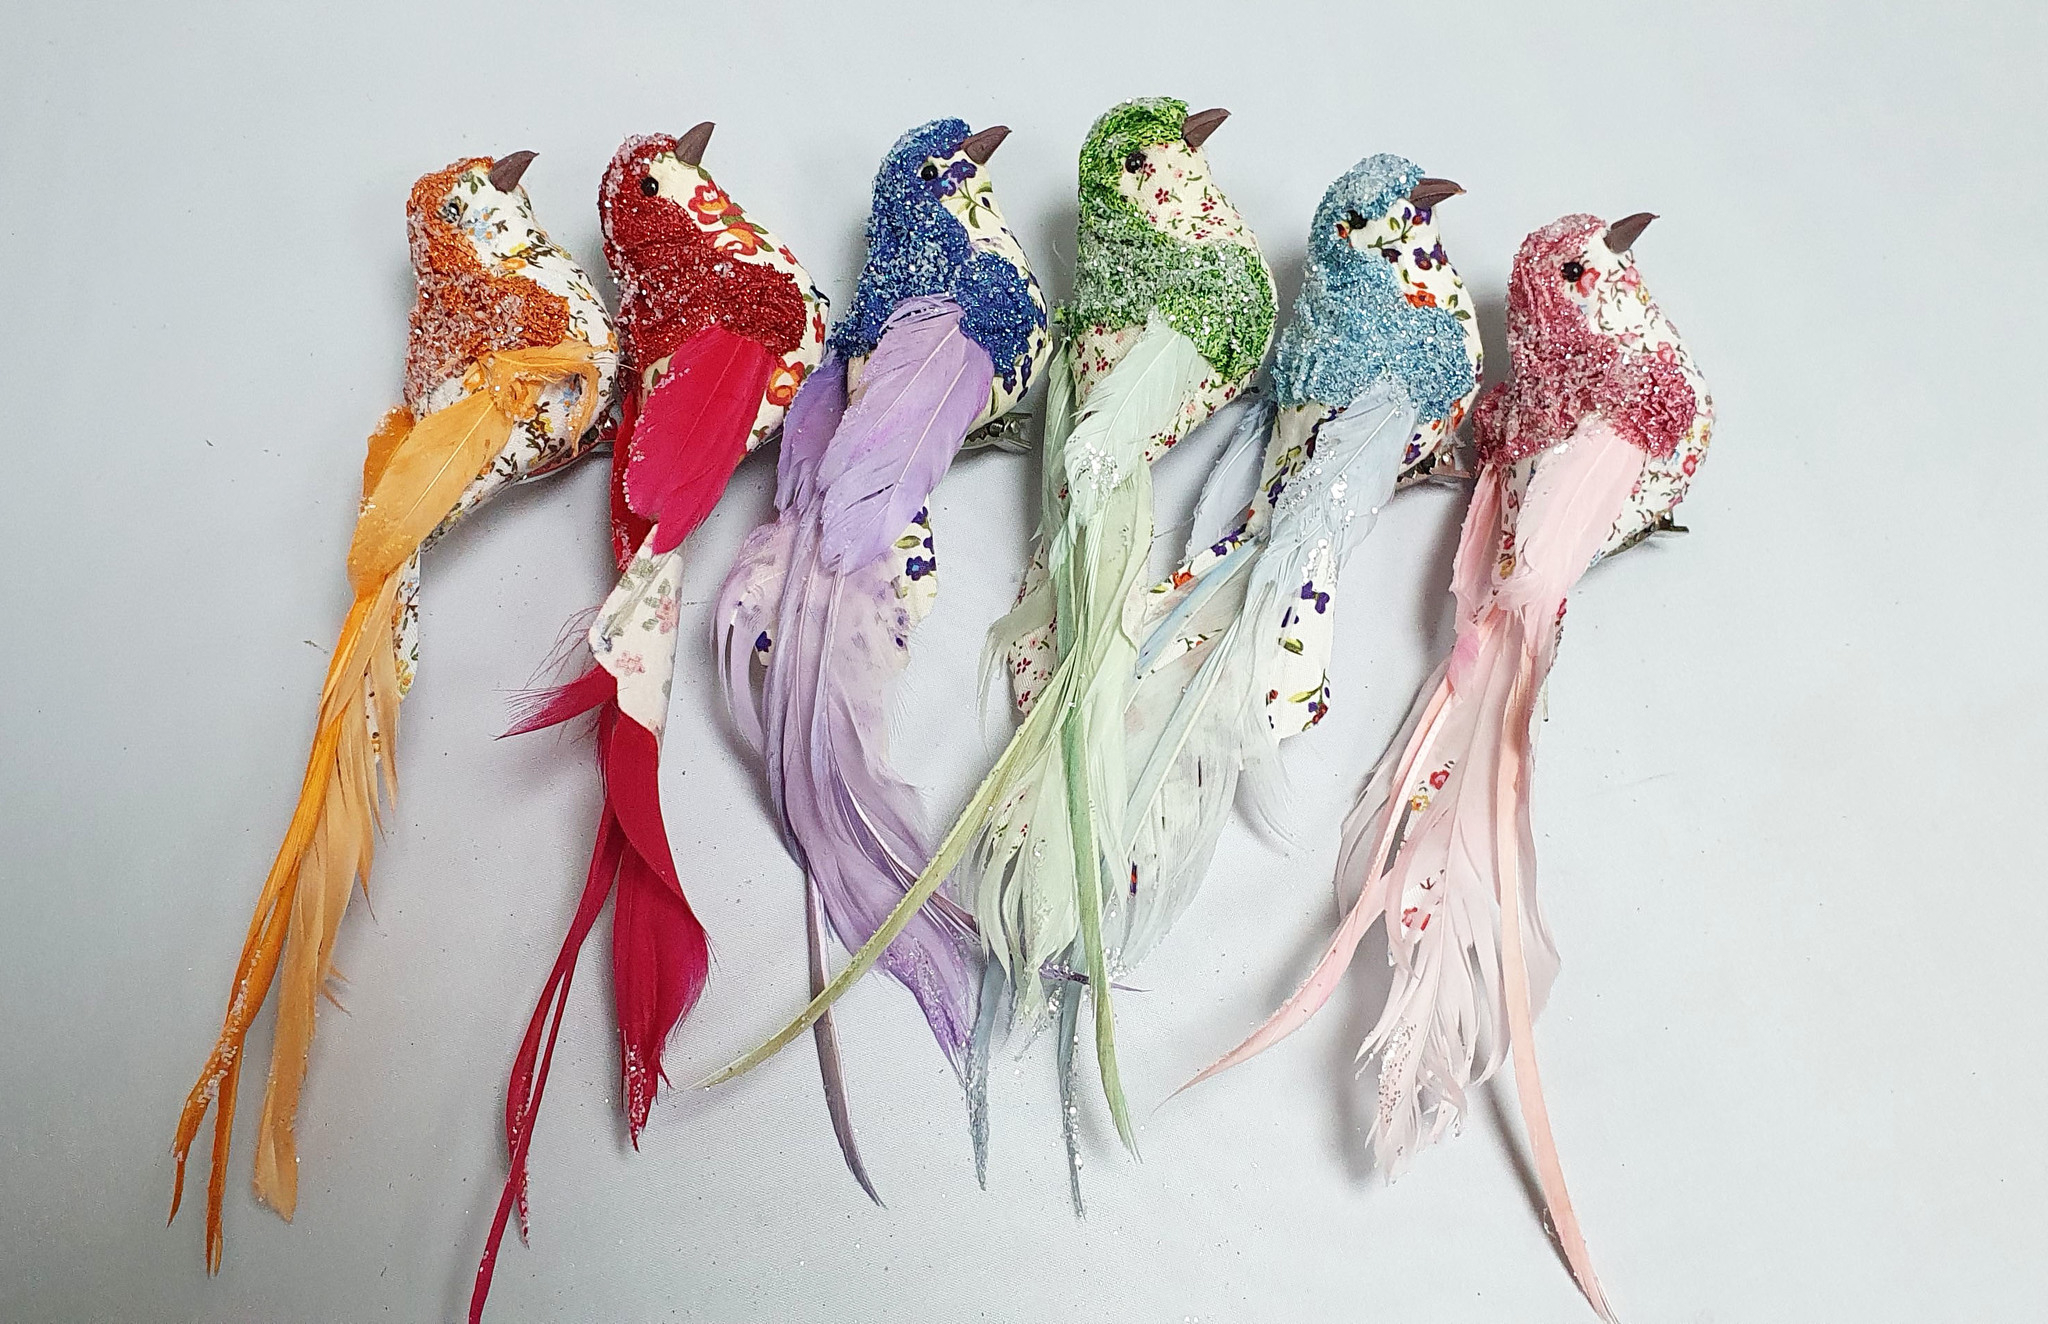
\includegraphics[width=7cm]{picture.jpg}
\hfill
\caption{Птички}
\label{figLeft}
\hfill
\begin{asy}
size(5cm);
path thebox = box((0,0),(1,1));
fill(thebox, blue);
draw(shift(.5,.5)*thebox,green+linewidth(5pt));
clip(thebox);
draw(shift(-.5,-.5)*thebox,red+linewidth(5pt));
\end{asy}
\hfill
\caption{Типо квадратики...}
\label{figRight}
\end{multicols}
\end{figure}



\end{document}